\section{Introduction to Computer vision}
\label{sec:introduction_to_computer_vision}

Assignments for \textit{BE1\_IntroComputerVision} practical.

\subsection{Basics}

\textbf{Question 1:}
\textit{Load and Display a grayscale image and a color image. How do you interpret the image coding under MatLab? What is the data type?}

\begin{figure}[H]
    \centering
    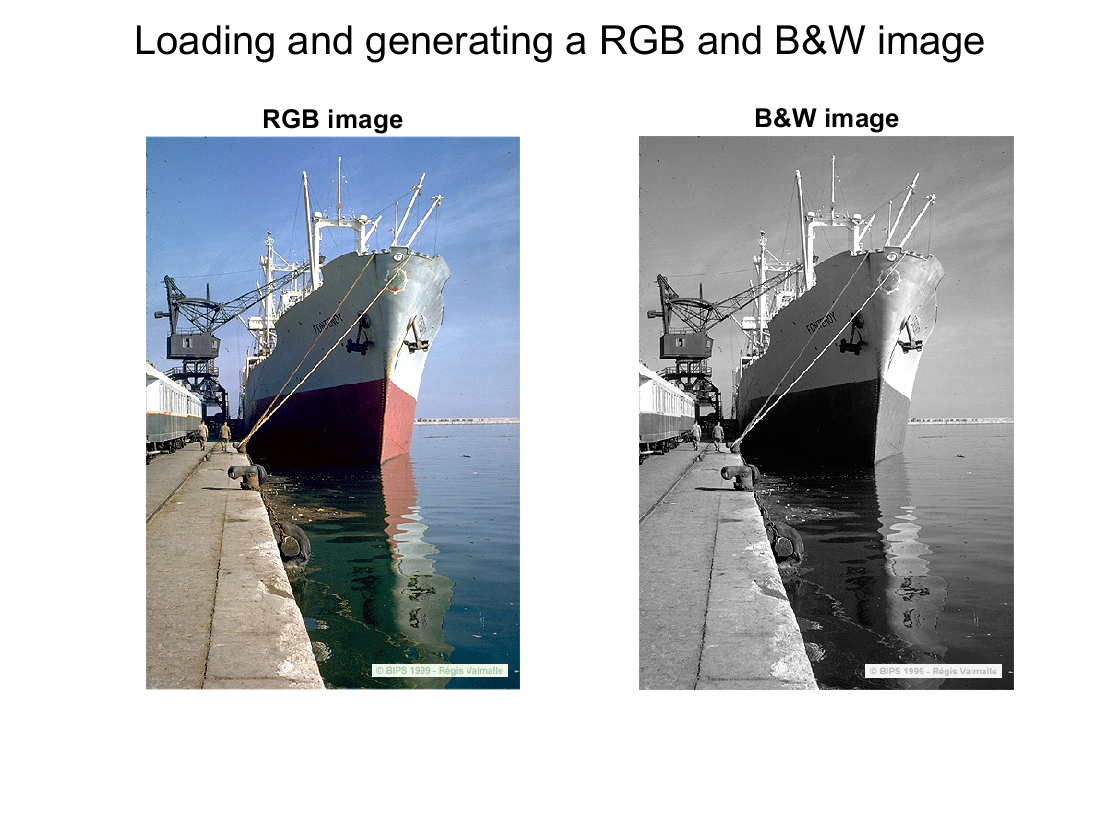
\includegraphics[width=0.5\linewidth]{Doc/Graphics/Part1_Question1.png}
    \label{fig:enter-label}
\end{figure}


\subsubsection{Greyscale Image Coding}

\textbf{Question 2:}
\textit{Build a matrix with a gradual value of intensity and an horizontal line with a constant value; the representative image is shown Fig. 1.}

\begin{figure}[H]
    \centering
    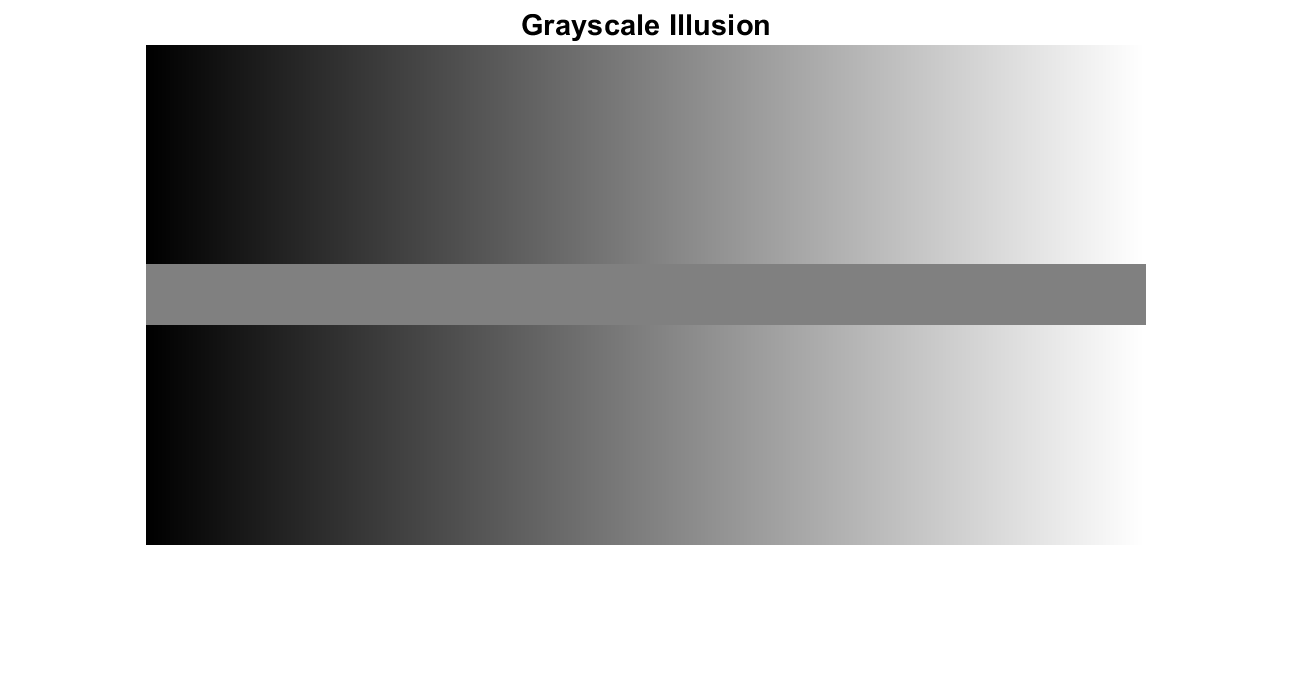
\includegraphics[width=0.5\linewidth]{Doc/Graphics/Part1_Question2.png}
    \label{fig:enter-label}
\end{figure}



\textbf{Question 3:}
\textit{Build a matrix of black \& white stripes, and with a rectangle and disk as shown Fig. 2. All parameters (size of stripes, size of rectangle, radius) should be easily modifiable.}

\begin{figure}[H]
    \centering
    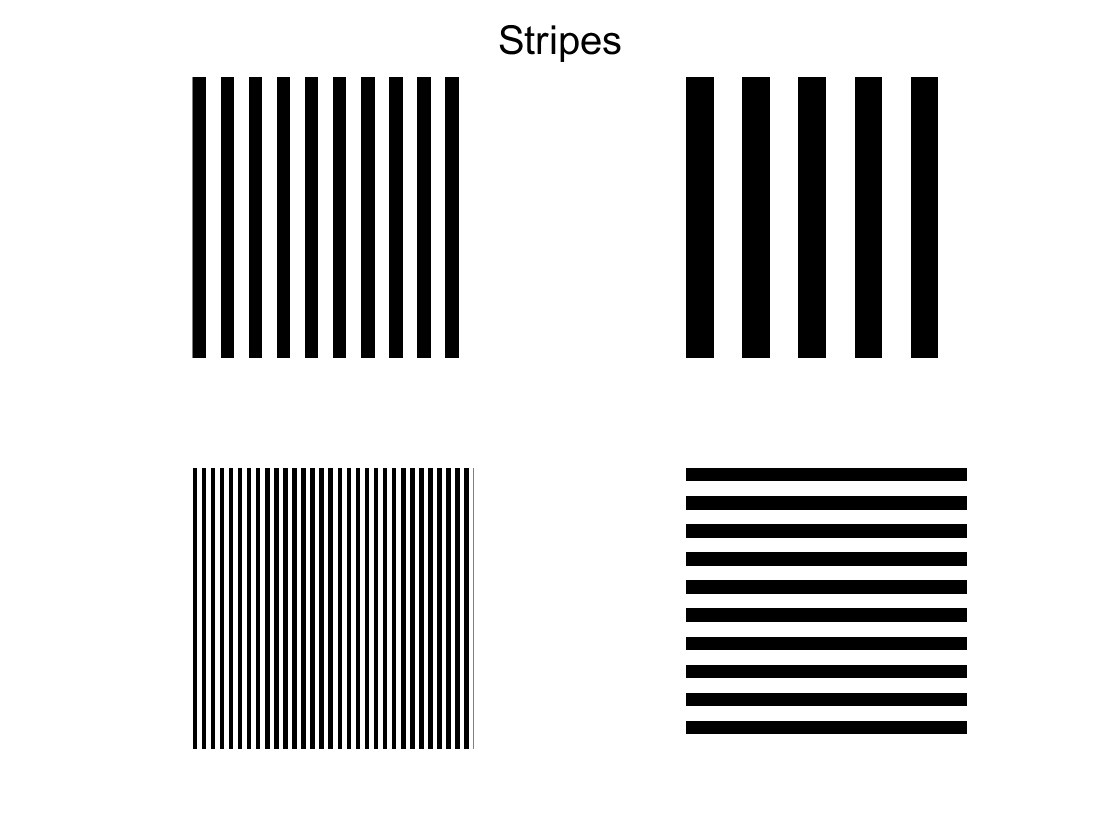
\includegraphics[width=0.75\linewidth]{Doc/Graphics/Part1_Question3a.png}
    \label{fig:enter-label}
\end{figure}

\begin{figure}[H]
    \centering
    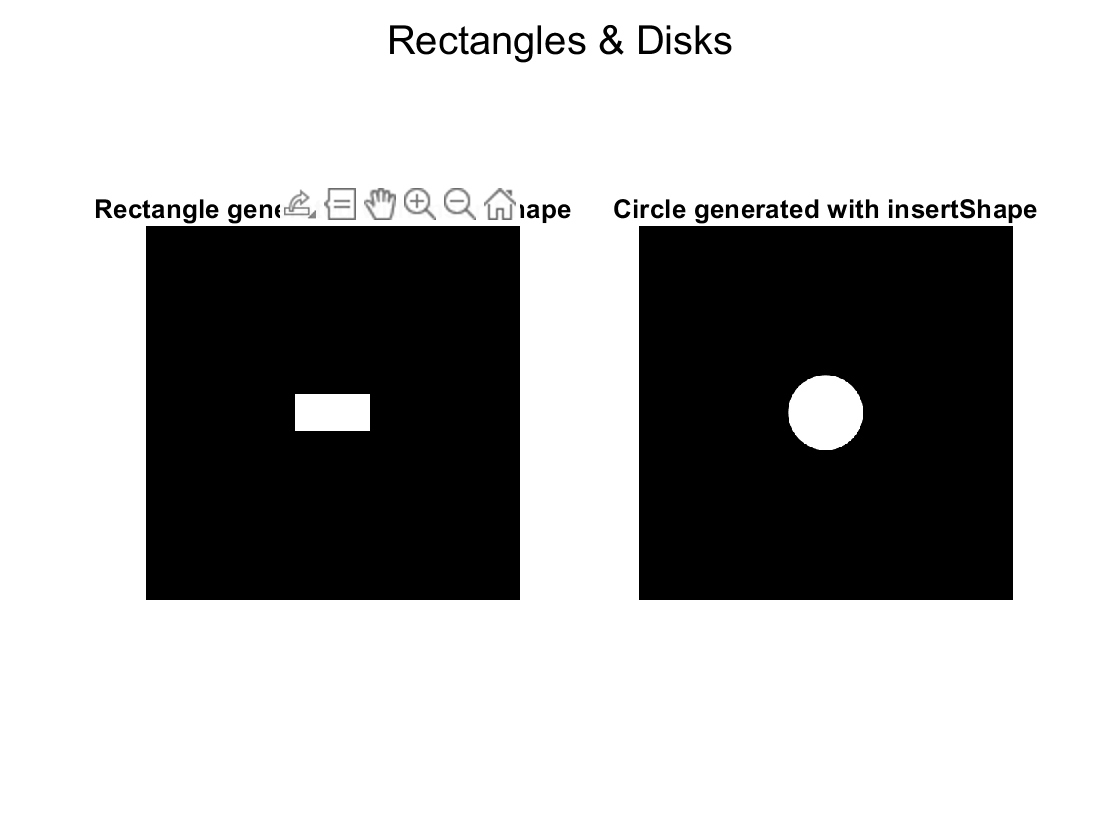
\includegraphics[width=0.5\linewidth]{Doc/Graphics/Part1_Question3b.png}
    \label{fig:enter-label}
\end{figure}



\subsubsection{Colour Image Coding}
\textbf{Question 4:}
\textit{Next, display Teinte.jpg and its red, green and blue components. Interpret and analyse. Same with oeil.jpg, cargo.jpg and CoulAdd.jpg.}

\begin{figure}[H]
    \centering
    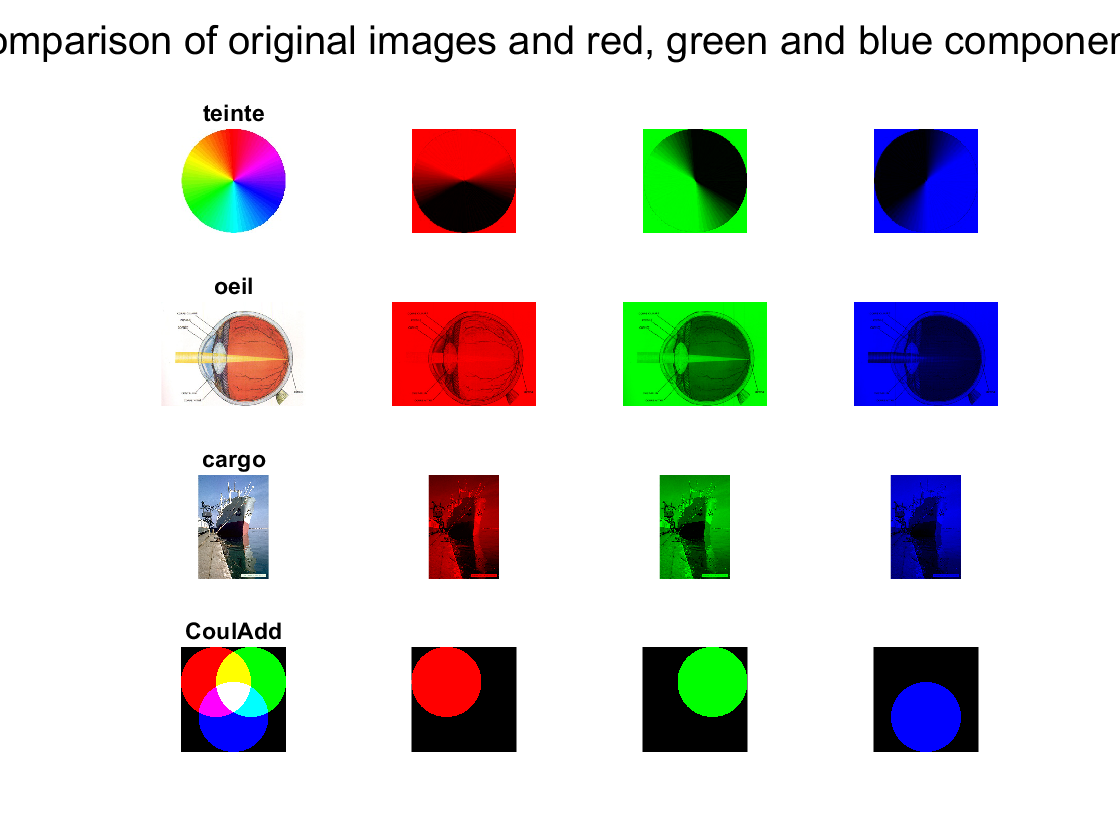
\includegraphics[width=\linewidth]{Doc/Graphics/Part1_Question4a.png}
    \label{fig:enter-label}
\end{figure}



\textbf{Question 5:}
\textit{Build and display the french flag. Build and display your flag.}

\begin{figure}[H]
    \centering
    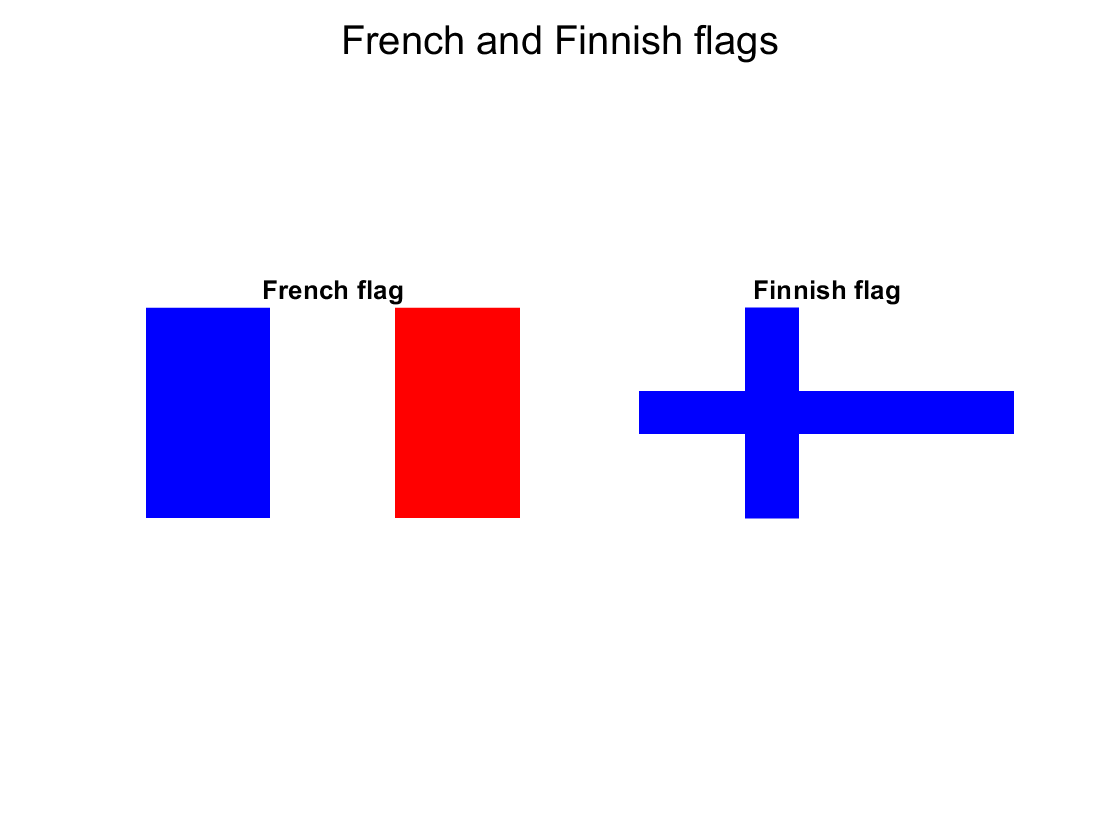
\includegraphics[width=0.5\linewidth]{Doc/Graphics/Part1_Question5.png}
    \label{fig:enter-label}
\end{figure}



\textbf{Question 6:}
\textit{Use the HSV code (with the command rgb2hsv and interpret images. How is the type of the new matrix? Build and display the image Fig. 4.}

\begin{figure}[H]
    \centering
    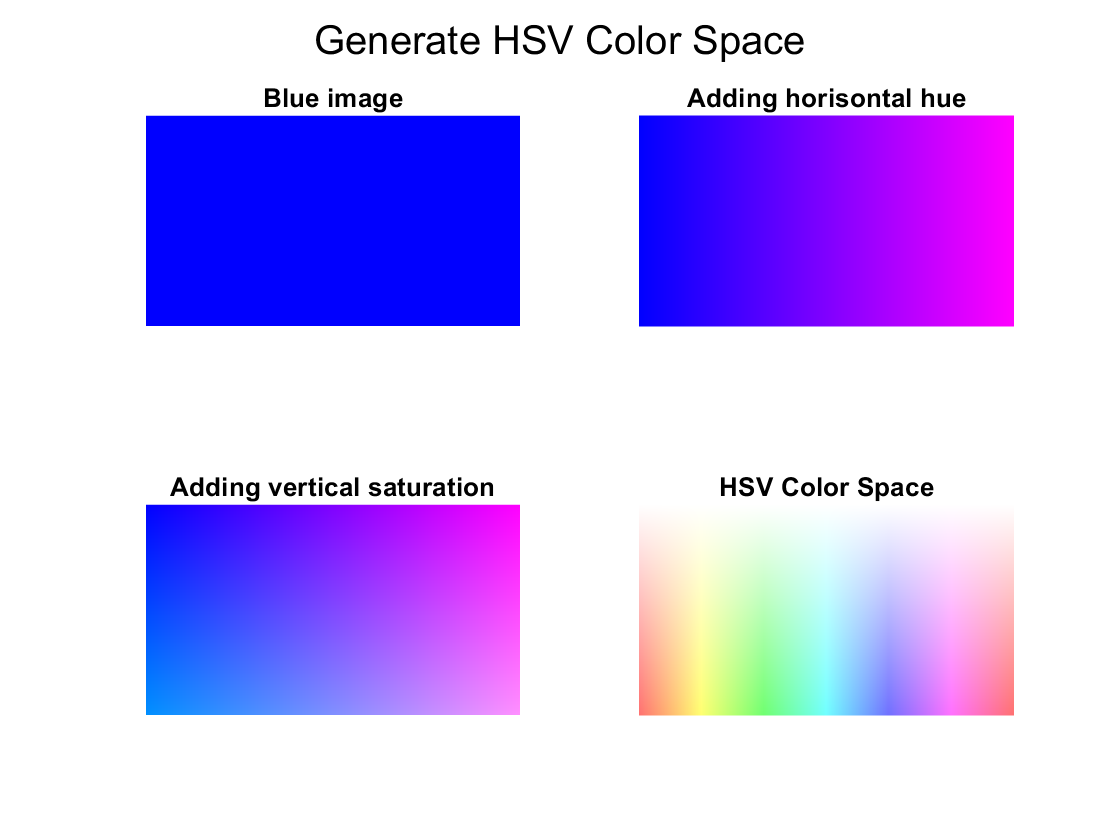
\includegraphics[width=0.75\linewidth]{Doc/Graphics/Part1_Question6a.png}
    \label{fig:enter-label}
\end{figure}

\begin{figure}[H]
    \centering
    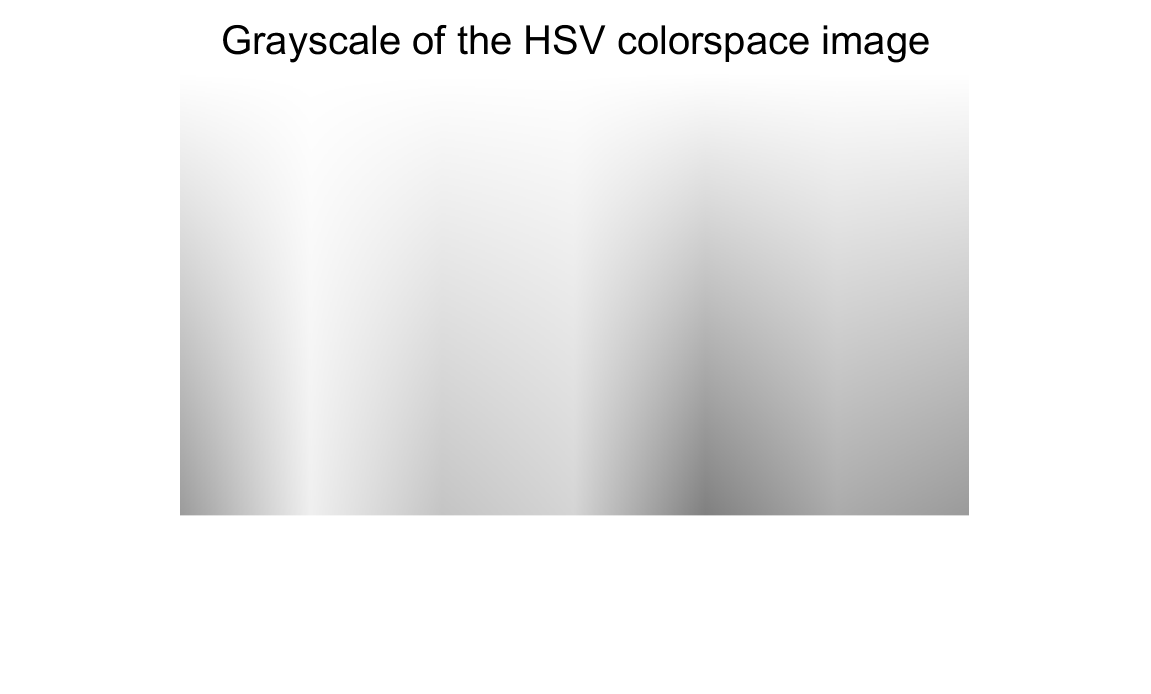
\includegraphics[width=0.5\linewidth]{Doc/Graphics/Part1_Question6b.png}
    \label{fig:enter-label}
\end{figure}



\textbf{Question 7:}
\textit{What are the values of $\alpha$, $\beta$ and $\gamma$?}




\textbf{Question 8:}
\textit{Load and display SpainBeach.png and isolate the beach.}

\begin{figure}[H]
    \centering
    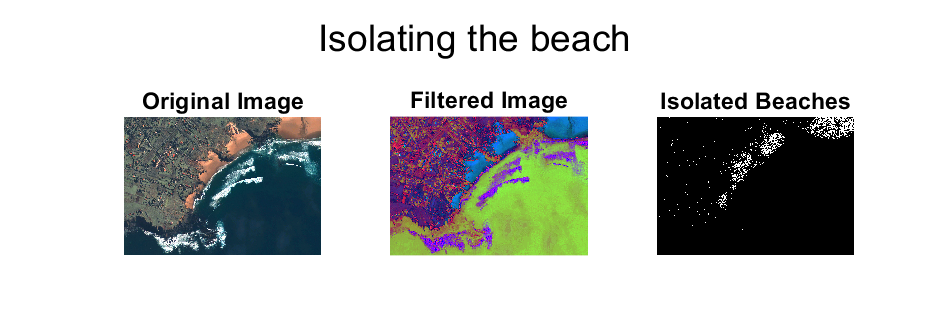
\includegraphics[width=0.5\linewidth]{Doc/Graphics/Part1_Question8.png}
    \label{fig:enter-label}
\end{figure}



\subsubsection{Histograms}
\textbf{Question 9:}
\textit{What is a histogram? What is the use? Display and interpret histograms of images.}




\textbf{Question 10:}
\textit{Work the mysterious images called Imagex.bmp and Imagexx.bmp.}




\subsubsection{Filtering}
\textbf{Question 11:}
\textit{Apply blur Filtering and Edge filtering on the Stripes images and on a ’real’ image. What are the main associated Kernels ?}



\textbf{Question 12:}
\textit{Thanks to successive filtering operators, isolate the main 5 stars of the image Etoile.png.}


\subsection{Fourier Transform}
\textbf{Question 13:}
\textit{Get the FT and analyze the spectrum if images with stripes (Fig. 2), rectangle and disks (Fig. 3).}



\textbf{Question 14:}
\textit{Blur the image with different kernels and interpret the spectrum.}



\textbf{Question 15:}
\textit{Write a program that extracts the specific field in the image Champs.jpg (see Fig. 5).}



% ~~~~~~~~~~~~~~~~~~~~~~~~~~~~~~~~
% Subsection: Deblurring
% ~~~~~~~~~~~~~~~~~~~~~~~~~~~~~~~~
\subsection{Deblurring}
\subsubsection{Linear Modelization}
\textbf{Question 16:}
\textit{Why do we have chosen this model? What are the limits of this model with respect to a single lens model?}



\textbf{Question 17:}
\textit{Compare the spectrums of the original image and of the blur image: what do you observe? Justify.}



\subsubsection{Blur Estimation}
\textbf{Question 18:}
\textit{Propose a cardinal sinus function that have the same zeros than H(u) (superpose the two functions). What conclusion could you give from these properties? Could you estimate T ?}


\textbf{Question 19:}
\textit{Estimate T.}




\subsubsection{Image Deblurring}

The following program allows to apply this process (Inverse Filtering -> Wiener Filtering):
\begin{lstlisting}
    SeuilMax = 11 ;
    hh = zeros(TailleImage);
    centre = [1 1] + floor(TailleImage/2) ;
    ext = (TailleFiltre-[1 1])/2;
    ligs = centre(1) + [-ext(1):ext(1)];
    cols = centre(2) + [-ext(2):ext(2)];
    
    h = ones(TailleFiltre)/prod(TailleFiltre);
    hh(ligs,cols) = h;
    hh = ifftshift(hh);
    
    H = fft2(hh);
    
    ind = find(abs(H)<(1/SeuilMax));
    H(ind) = (1/SeuilMax)*exp(j*angle(H(ind)));
    
    G = ones(size(H))./H;
    
    (...)
\end{lstlisting}


\textbf{Question 20:}
\textit{Complete this program (only 2 lines!) to process inverse filtering method.}



\textbf{Question 21:}
\textit{What’s happen with the image marcheur.jpg ?}